%
%
%
\exercises

%%%%%%%%%%%%%%%%%%%%%%%%%%%%%%%%%%%%%%%%%%%%%%%%%%%%%%%%%%%%%%%%%%%%%%%%
% Lists
%
\begin{exercise}{union-list}
Suppose you are given the following definition of a list type.

\begin{ocaml}
type 'a mylist = Nil | Cons of 'a * 'a mylist
\end{ocaml}

\begin{enumerate}
\item Write a function \hbox{\lstinline/map : ('a -> 'b) -> 'a mylist -> 'b mylist/}, where

\lstinline!map $f$ [$x_0$; $x_1$; $\cdots$; $x_n$] = [$f$ $x_0$; $f$ $x_1$; $\cdots$; $f$ $x_n$]!.

\begin{answer}\ifanswers
This is a non-tail-recursive version of \hbox{\lstinline/map/}.

\begin{ocaml}
let rec map f = function
   Nil -> Nil
 | Cons (h, t) -> Cons (f h, map f t)
\end{ocaml}
%
For a tail-recursive version, we collect the list in reverse order.

\begin{ocaml}
let rec rev accum = function
   Nil -> accum
 | Cons (h, t) -> rev (Cons (h, accum)) t

let map f l =
   let rec loop accum = function
      Nil -> rev Nil accum
    | Cons (h, t) -> loop (Cons (f h, accum)) t
   in
      loop Nil l
\end{ocaml}
\fi\end{answer}

\item Write a function \hbox{\lstinline/append : 'a mylist -> 'a mylist -> 'a mylist/}, where

\lstinline!append [$x_1$; $\cdots$; $x_n$] [$x_{n + 1}$; $\cdots$; $x_{n + m}$] = [$x_1$; $\cdots$; $x_{n + m}$]!.

\begin{answer}\ifanswers
We give the tail-recursive version, using the function \hbox{\lstinline/rev/} as defined above.
\begin{ocaml}
let append l1 l2 =
   let rec loop l2 = function
      Cons (h, t) -> loop (Cons (h, l2)) t
    | Nil -> l2
   in
      loop l2 (rev l1)
\end{ocaml}
\fi\end{answer}
\end{enumerate}
\end{exercise}

%%%%%%%%%%%%%%%%%%%%%%%%%%%%%%%%%%%%%%%%%%%%%%%%%%%%%%%%%%%%%%%%%%%%%%%%
% Unary
%
\begin{exercise}{union-unary}
A type of unary (base-1) natural numbers can be defined as follows,

\begin{ocaml}
type unary_number = Z | S of unary_number
\end{ocaml}
%
where \hbox{\lstinline/Z/} represents the number zero, and if $i$ is a unary number, then \hbox{\lstinline/S $i$/}
is $i + 1$.  For example, the number 5 would be represented as \hbox{\lstinline/S (S (S (S (S Z))))/}.

\begin{enumerate}
\item Write a function to add two unary numbers.  What is the complexity of your function?

\begin{answer}\ifanswers
To add two numbers we use the following equivalences.

\begin{eqnarray*}
i + 0 & = & i\\
i + (j + 1) & = & (i + 1) + j
\end{eqnarray*}
%
This gives us the following loop.

\begin{ocaml}
let rec add i = function
   S j -> add (S i) j
 | Z -> i
\end{ocaml}
%
The time complexity of the expression \hbox{\lstinline/add $n$ $m$/} is $O(m)$.
\fi\end{answer}

\item Write a function to multiply two unary numbers.

\begin{answer}\ifanswers
We can multiply two numbers by repeated summing.

\begin{ocaml}
let mul n m =
   let rec loop sum = function
      Z -> sum
    | S m -> loop (add sum n) m
   in
      sum Z m
\end{ocaml}
\fi\end{answer}
\end{enumerate}
\end{exercise}

%%%%%%%%%%%%%%%%%%%%%%%%%%%%%%%%%%%%%%%%%%%%%%%%%%%%%%%%%%%%%%%%%%%%%%%%
% Comparison
%
\begin{exercise}{union-compare}
Suppose we have the following definition for a type of small numbers.

\begin{ocaml}
type small = Four | Three | Two | One
\end{ocaml}
%
The builtin comparison \hbox{\lstinline/(<)/} orders the numbers in reverse order.

\begin{ocaml}
# Four < Three;;
@
\begin{topoutput}
- : bool = true
\end{topoutput}
@
\end{ocaml}
%
\begin{enumerate}
\item
Write a function \hbox{\lstinline/lt_small : small -> small -> bool/} that orders the numbers in the
normal way.

\begin{answer}\ifanswers
The comparison can be implemented as a pattern matching on the pair of numbers to be compared.

\begin{ocaml}
let lt_small i j =
   match i, j with
      Zero, (One | Two | Three)
    | One, (Two | Three)
    | Two, Three ->
         true
    | _ ->
         false
\end{ocaml}
%
However, this implementation has poor style because of the wildcard matching \hbox{\lstinline/_ -> false/}.
If another number, like \hbox{\lstinline/Five/}, is added to the type, the implementation of
\hbox{\lstinline/lt_small/} must be changed.  It is better to avoid the use of wildcards.

\begin{ocaml}
let lt_small i j =
   match i, j with
      Zero, (One | Two | Three)
    | One, (Two | Three)
    | Two, Three ->
         true
    | Zero, Zero
    | One, (Zero | One)
    | Two, (Zero | One | Two)
    | Three, (Zero | One | Two | Three) ->
         false
\end{ocaml}
\fi\end{answer}

\item

Suppose the type \hbox{\lstinline/small/} defines $n$ small integers.  How does the size of your code depend on $n$?

\begin{answer}\ifanswers
With the implementation style above, the code is quadratic $O(n^2)$.

One way to reduce the code size in this case is to map the type onto a linear subrange of the
integers, then use the builtin comparison.

\begin{ocaml}
let index_of_small = function
   Four -> 4
 | Three -> 3
 | Two -> 2
 | One -> 1

let lt_small i j = index_of_small i < index_of_small j
\end{ocaml}
\fi\end{answer}
\end{enumerate}
\end{exercise}

%%%%%%%%%%%%%%%%%%%%%%%%%%%%%%%%%%%%%%%%%%%%%%%%%%%%%%%%%%%%%%%%%%%%%%%%
% Expressions
%
\begin{exercise}{evaluator}
We can define a data type for simple arithmetic expressions as follows.

\begin{ocaml}
type unop = Neg
type binop = Add | Sub | Mul | Div
type exp =
   Constant of int
 | Unary of unop * exp
 | Binary of exp * binop * exp
\end{ocaml}
%
Write a function \hbox{\lstinline/eval : exp -> int/} to \emph{evaluate} an expression, performing the
calculation to produce an integer result.

\begin{answer}\ifanswers
\begin{ocaml}
let rec eval = function
   Constant i -> i
 | Unary (Neg, e) -> -(eval e)
 | Binary (e1, op, e2) ->
      let i = eval e1 in
      let j = eval e2 in
         match op with
            Add -> i + j
          | Sub -> i - j
          | Mul -> i * j
          | Div -> i / j
\end{ocaml}
\fi\end{answer}
\end{exercise}

%%%%%%%%%%%%%%%%%%%%%%%%%%%%%%%%%%%%%%%%%%%%%%%%%%%%%%%%%%%%%%%%%%%%%%%%
% Dictionary
%
\begin{exercise}{dict2}
In Exercise~\ref{exercise:dict1} we defined the data structure called a \emph{dictionary}.  Another
way to implement a dictionary is with tree, where each node in the tree has a label \emph{and} a
value.  Implement a polymorphic dictionary, \hbox{\lstinline/('key, 'value) dictionary/}, as a tree with
the three dictionary operations.

\begin{ocaml}
empty : ('key, 'value) dictionary
add   : ('key, 'value) dictionary -> 'key -> 'value -> ('key, 'value) dictionary
find  : ('key, 'value) dictionary -> 'key -> 'value
\end{ocaml}

\begin{answer}\ifanswers
The central difference between a set and a dictionary is that a node has both a \hbox{\lstinline/'key/} and
a \hbox{\lstinline/'value/}.  The \hbox{\lstinline/add/} function is similary to \hbox{\lstinline/insert/}, and the
\hbox{\lstinline/find/} function is similar to \hbox{\lstinline/mem/}.

\begin{ocaml}
type ('key, 'value) dictionary =
   Node of 'key * 'value * ('key, 'value) dictionary * ('key, 'value) dictionary
 | Leaf

let empty = Leaf

let rec add dict key value =
   match dict with
      Leaf -> Node (key, value, Leaf, Leaf)
    | Node (key', value', left, right) ->
         if key < key' then
            Node (key', value', add left key value, right)
         else if key > key' then
            Node (key', value', left, add right key value)
         else (* key = key' *)
            Node (key, value, left, right)
      
let rec find dict key =
   match dict with
      Leaf ->
         raise Not_found
    | Node (key', value, left, right) ->
         if key < key' then
            find left key
         else if key > key' then
            find right key
         else (* key = key' *)
            value
\end{ocaml}
\fi\end{answer}
\end{exercise}

%%%%%%%%%%%%%%%%%%%%%%%%%%%%%%%%%%%%%%%%%%%%%%%%%%%%%%%%%%%%%%%%%%%%%%%%
% Graph
%
\begin{exercise}{graph}
A \emph{graph} $(V, E)$ has a set of \emph{vertices} $V$ and a set of \emph{edges} $E \subseteq
V \times V$, where each edge $(v_1, v_2)$ is a pair of vertices.  In a \emph{directed} graph, each
edge is an arrow from one vertex to another.  For example, for the graph below, the set of vertices
is $V = \{ 1, 2, 3, 4 \}$, and the set of edges is $\{ (1, 2), (1, 3), (1, 4), (2, 4), (3, 4) \}$.

\begin{center}
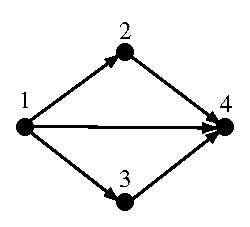
\includegraphics[scale=0.5]{graph1}
\end{center}
%
One way to represent a graph is with a dictionary \hbox{\lstinline/(vertex, vertex list) dictionary/} where
each entry in the dictionary lists the outgoing edges from that vertex.
Assume the following type definitions.

\begin{ocaml}
type vertex = int
type graph = (vertex, vertex list) dictionary
\end{ocaml}
%
Write a function \hbox{\lstinline/reachable : graph -> vertex -> vertex -> bool/}, where
\hbox{\lstinline/reachable graph v1 v2/} is \hbox{\lstinline/true/} iff vertex \hbox{\lstinline/v2/} is
reachable from \hbox{\lstinline/v1/} by following edges only in the forward direction.  Your algorithm should
terminate on all inputs.

\begin{answer}\ifanswers
To ensure that the algorithm terminates, we need to keep track of which vertices have already been
visited using a set \hbox{\lstinline/visited/} of vertices that have already been visited.  The
reachability test can be performed by a depth-first-search.

\begin{ocaml}
let reachable graph v1 v2 =
   let rec search visited v =
      if v = v2 then
         true
      else if set_mem visited v then
         false
      else
         search_list (set_insert visited v) (dict_find graph v)
   and search_list visited = function
      v :: vl -> search visited v || search_list visited vl
    | [] -> false
   in
      search set_empty v1
\end{ocaml}
\fi\end{answer}
\end{exercise}

%%%%%%%%%%%%%%%%%%%%%%%%%%%%%%%%%%%%%%%%%%%%%%%%%%%%%%%%%%%%%%%%%%%%%%%%
% Comparison
%
\begin{exercise}{set-compare}
Consider the function \hbox{\lstinline/insert/} for unbalanced, ordered, binary trees in
Section~\refsection{unbalanced-btree}.  One potential problem with this implementation is that it
uses the builtin comparison \hbox{\lstinline/(<)/}.  Rewrite the definition so the it is parameterized by a
comparison function that, given two elements, returns on of three values
%
\hbox{\lstinline/type comparison = LessThan | Equal | GreaterThan/}.
%
The expression \hbox{\lstinline/insert compare x tree/} inserts an element \hbox{\lstinline/x/} into the tree
\hbox{\lstinline/tree/}.  The type is
%
\hbox{\lstinline/insert : ('a -> 'a -> comparison) -> 'a -> 'a tree -> 'a tree/}.

\begin{answer}\ifanswers
The principal change is to use pattern matching instead of the conditional.

\begin{ocaml}
let rec insert compare x = function
   Leaf -> Node (x, Leaf, Leaf)
 | Node (y, left, right) as node ->
     match compare x y with
        LessThan -> Node (y, insert compare x left, right)
      | Equal -> node
      | GreaterThan -> Node (y, left, insert compare x right)
\end{ocaml}
\fi\end{answer}
\end{exercise}

%%%%%%%%%%%%%%%%%%%%%%%%%%%%%%%%%%%%%%%%%%%%%%%%%%%%%%%%%%%%%%%%%%%%%%%%
% Heaps
%
\begin{exercise}{heap}
A \emph{heap} of integers is a data structure supporting the following operations.

\begin{itemize}
\item \lstinline!makeheap : int -> heap!: create a heap containing a single element,
\item \lstinline!insert : heap -> int -> heap!: add an element to a heap; duplicates are allowed,
\item \lstinline!findmin : heap -> int!: return the smallest element of the heap.
\item \lstinline!deletemin : heap -> heap!: return a new heap that is the same as the original, without the smallest element.
\item \lstinline!meld : heap -> heap -> heap!: join two heaps into a new heap containing the elements of both.
\end{itemize}
%
A heap can be represented as a binary tree, where for any node $a$, if $b$ is a child node of $a$,
then $\ms{label}(a) \le \ms{label}(b)$.  The order of children does not matter.  A \emph{pairing heap} is a
particular implementation where the operations are performed as follows.

\begin{itemize}
\item \lstinline!makeheap i!: produce a single-node tree with \hbox{\lstinline/i/} at the root.
\item \lstinline!insert h i = meld h (makeheap i)!.
\item \lstinline!findmin h!: return the root label.
\item \lstinline!deletemin h!: remove the root, and \hbox{\lstinline/meld/} the subtrees.
\item \lstinline!meld h1 h2!: compare the roots, and make the heap with the larger element a subtree of the other.
\end{itemize}
%
\begin{enumerate}
\item
Define a type \hbox{\lstinline/heap/} and implement the five operations.

\begin{answer}\ifanswers
\begin{ocaml}
type heap = Node of int * heap list

let makeheap i = Node (i, [])

let meld (Node (i1, c1) as h1) (Node (i2, c2) as h2) =
   if i1 < i2 then
      Node (i1, h2 :: c1)
   else
      Node (i2, h1 :: c2)

let insert h i =
   meld h (makeheap i)

let findmin (Node (i, _)) =
   i

let deletemin = function
   Node (_, []) -> raise (Invalid_argument "deletemin")
 | Node (_, [h]) -> h
 | Node (_, h :: t) ->
     let rec meld_all h = function
        x :: t -> meld_all (meld h x) t
      | [] -> h
     in
        meld_all h t
\end{ocaml}
\fi\end{answer}

\item A \emph{heap sort} is performed by inserting the elements to be sorted into a heap,
then the values are extracted from smallest to largest.  Write a function
\hbox{\lstinline/heap_sort : int list -> int list/} that performs a heap sort,
where the result is sorted from largest to smallest.

\begin{answer}\ifanswers
\begin{ocaml}
let insert_list heap = function
   i :: elements -> insert_list (insert heap i) elements
 | [] -> heap

let heap_sort = function
   [] -> []
 | i :: elements ->
     let rec loop sorted heap =
        match heap with
           Node (i, []) -> i :: sorted
         | _ -> loop (findmin heap :: sorted) (deletemin heap)
     in
        loop [] (insert_list (makeheap i) elements)
\end{ocaml}
\fi\end{answer}
\end{enumerate}
\end{exercise}

% -*-
% Local Variables:
% Mode: LaTeX
% fill-column: 100
% TeX-master: "paper"
% TeX-command-default: "LaTeX/dvips Interactive"
% End:
% -*-
% vim:tw=100:fo=tcq:
